% Das gesetzt von Conway [Seite 39 EWolff2016:Microservices]
\chapter[Grundlagen]{Allgemeine Grundlagen zur Verwendung von Service-orientierten Systemen}
\label{chap:grundlagen}
Software zu entwickeln ist nicht immer einfach. Umso größer diese ist, umso mehr Probleme können auftreten. Es bedarf einer genauen Planung und Verständnis von Infrastruktur um eine Software mit allen Anforderungen, zufriedenstellend zu implementieren. 

Vor allem wenn es um die Weiterentwicklung und Wartung von Software geht, können große Probleme auftreten. Wurde die Architektur nicht gut gewählt oder schlecht umgesetzt, kann es das weitere Vorgehen stark beeinträchtigen, bis hin zum unmöglich machen. Es wurden daher Software-Architekturen entwickelt, welche flexibel und einfacher zu ändern sind. Außerdem kann in diesen Architekturen neue Funktionen deutlich schneller hinzugefügt werden.

\section{Die Service-orientierte Architektur}
\label{sec:architektur}
Diese Architekturen zielen, wie der Name schon sagt, auf eigenständige Dienste ab, welche durch verschiedene Kommunikationskanäle miteinander kommunizieren können und dadurch die gewünschten Geschäftsprozesse abbilden. 
\begin{quotation}
    \frqq Ein Programm soll nur eine Aufgabe erledigen, und das soll es gut machen\flqq \cite[S. 2]{EWolff2015:ContinuouosDelivery}
\end{quotation}
Anstatt eine einzige große Anwendung ein zu setzten, setzt man auf viele kleine, verteile, autarke Anwendungen, welche jeweils Schnittstellen nach außen hin anbieten damit der Service genutzt werden kann. Diese Schnittstellen können unter anderem durch REST-HTTP angeboten werden.
Durch die verteilten Anwendungen kann das System auch dann noch funktionieren, wenn einzelne Dienste nicht verfügbar sind, jedoch bringt es ebenfalls die typischen Probleme von Verteilten Anwendungen mit sich.

\section{Verteilte Systeme}
\label{sec:VerteilteAnwendungen}
\begin{quotation}
    \frqq Ein verteiltes System ist eine Ansammlung unabhängiger Computer, die den Benutzer wie ein einzelnes kohärentes System erscheinen.\flqq\cite[S. 19]{tanenbaum:VerteilteSysteme}
\end{quotation}
Im Falle von Service-orientierten Architekturen wird das System auf mehrere eigenständige Computer bzw. Anwendungen aufgeteilt. Ein Vorteil von verteilten Systemen ist, dass sie zum einen sehr dynamisch und schnell anpassbar sind, zum anderen jedoch auch die Komplexität von Software in einzelne Teile zerbricht, wodurch zum Beispiel eine entfernte Präsentation möglich ist.
Jedoch entstehen dadurch Probleme, welche in monolithischen Systemen/Anwendungen nicht vorhanden sind.
\\\\
Eines der wichtigsten und größten Probleme besteht dabei in der Kommunikation. Zum einen muss diese gewährleistet werden, zum anderen jedoch auch in angemessener Zeit erfolgen. Dabei muss ebenfalls darauf geachtet werden, dass Nachrichten erfolgreich zugestellt werden, selbst wenn einzelne Dienste nicht erreichbar sind.
\\\\
Ein weiteres Problem besteht darin, zu erkennen wenn ein Dienst ausgefallen ist. Meistens erkennt man dies nur dadurch, dass ein Teilsystem nicht funktioniert. Das ausgefallene System zu identifizieren stellt sich, wenn keine entsprechenden Vorkehrungen getroffen wurden, als schwer heraus. Zudem kann eine lange Zeit vergehen, bis das Unternehmen merkt, dass ein System ausgefallen ist.

\subsection{Domain-Driven Design und Bounded Context}
\label{sec:boundedContext}
Domain-Driven Design (DDD) beschreibt dabei die Herangehensweise zur Modellierung von komplexer Software. Dabei ist die Modellierung maßgeblich an die umzusetzende Fachlichkeit gebunden und wird durch diese beeinflusst. Das Ziel jeglicher Software ist es, eine bestimmte Anwendungsdomäne zu unterstützen. Damit dies erfolgreich geschieht, muss Software harmonisch und in höchster Form Interoperabel zur Anwendungsdomäne sein. Domain-Driven Design soll genau diesen Fall unterstützen.
\\\\
Arbeitet man mit Service-Orientierten Architekturen, versucht man Fachlichekomponenten, welche zu einem bestimmten Kontext gehören, möglichst nahe beieinander zu halten. Man spricht hierbei von \textit{Bounded Context}. 
\begin{quotation}
    \frqq Bounded Context ist ein zentrales Muster in Domain-Driven Design.[..] DDD arbeitet mit großen Modellen, indem es diese in kleine verschiedene zusammengehörige Kontexte unterteilt und auf ihre Wechselwirkung unterteilt.\flqq \cite{mfowler:BoundedContext}
\end{quotation}

\begin{figure}[htb]
    \centering 
    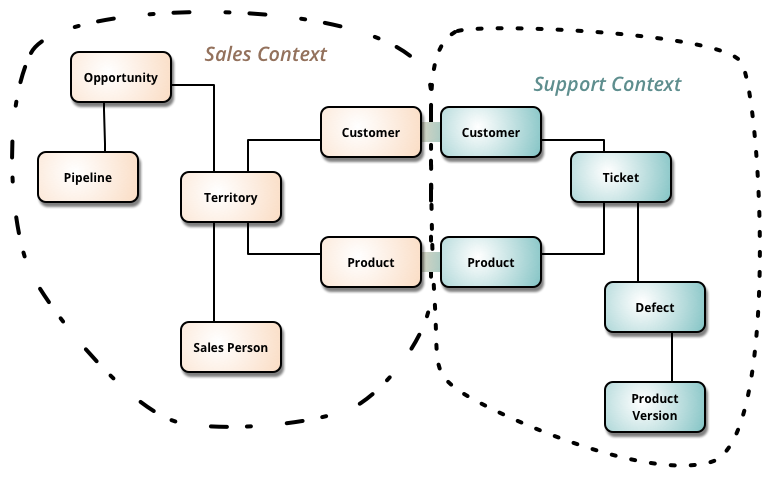
\includegraphics[width=\linewidth]{content/images/BoundedContext}\
    \quelle\url{http://martinfowler.com/bliki/BoundedContext.html}
    \caption[Bounded Context]{Bounded Context\\}
    \label{fig:BoundedContext}  
\end{figure} 
In dieser Grafik wird noch einmal der Begriff Bounded Context genauer verdeutlicht. Es existieren zwei eigenständige Prozesse. Auf der linken Seite der Sales Kontext und auf der rechten Seite der Support Kontext. Jeder Kontext besitzt verschiedene Services, welche benötigt werden um den Prozess durchführen zu können. Lediglich zwischen den \textit{Customer} und \textit{Product} Services besteht eine Verbindung der beiden Prozesse.

\subsection{Das Gesetzt von Conway}
\label{subsec:conway}
Spricht man von Service-orientierten Architekturen, sollte das \glqq Gesetzt von Conway\grqq\ nicht fehlen, da es Prinzipien beschreibt, nach denen Unternehmens-Architektur entworfen wird.
\\\\
Melvin Conway ist ein amerikanischer Informatiker und formulierte seine Beobachtungen bezüglich der Kommunikationsstrukturen und Organisationen innerhalb eines Unternehmens. Seine Beobachtung, auch \glqq Gesetzt von Conway\grqq\ genannt lautet wie folgt:
\begin{center}
    \textit{Organisationen, die Systeme designen, können nur solche Designs entwerfen, welche die Kommunikationsstruktur dieser Organisationen abbilden.}
\end{center}

Conway möchte damit ausdrücken, dass die internen Kommunikationswege wichtig bei der Planung der Architektur ist. Jedes Team innerhalb einer Organisation trägt bei der Entwicklung der Architektur bei. Wird eine Schnittstelle zwischen zwei Teams benötigt, so müssen diese Teams auch kommunizieren können. Dabei müssen Kommunikationswege nicht immer offiziell sein. Oft gibt es informelle Kommunikationsstrukturen, die ebenfalls in diesem Kontext betrachtet werden können.
\\\\
Service-orientierte Systeme arbeiten nach dem gleichen Prinzip. Dienste in diesen Systemen sind eigenständig und müssen, damit daraus eine Funktionierende Anwendung bzw. System wird, müssen diese unter einander problemlos kommunizieren können.

\subsection{Synchrone vs Asynchrone Kommunikation}
\label{subsec:KommunikationASynchrone}
Die Kommunikation ist ein zentraler Bestandteil von Verteilten Systemen. Ohne Kommunikation kann kein Verteiltes System arbeiten. Der Ausfall eines Dienstes oder eines Kommunikationsweg hat die Folge, dass das System nicht mehr ordnungsgemäß arbeiten kann. Daher müssen Vorkehrungen getroffen werden, damit auch in diesem Falle das System funktioniert. Es muss grundlegend zwischen zwei Kommunikationsarten entschieden werden.
\\\\
Eine Kommunikationsart ist die Synchrone. Dabei werden Nachrichten zwischen zwei Anwendungen in Echtzeit versendet und empfangen. Ein Nachrichtenspeicher existiert hierbei nicht, wodurch Nachrichten verloren gehen, wenn sie nicht empfangen werden können. Die einzige Möglichkeit Fehler dieser Art abzufangen, ist es die aktuelle Aktion abzubrechen.
\\\\
Eine weitere Kommunikationsart ist die Asynchrone. Anders als bei der Synchronen, wird bei der Asynchronen Kommunikation ein Nachrichtenspeicher verwendet, welcher die Nachrichten entgegen nimmt und an den eigentlichen Empfänger weiterleitet. Ist der Empfänger nicht erreichbar, werden die Nachrichten solange gespeichert, bis der Empfänger sie abruft.

\section{Orchestration vs Choreographie}
\label{sec:OrchestrationVsChoregraphie}

\subsection*{Orchestration}
\label{subsec:orchestration}
Bei der Orchestration handelt es sich um eine Komposition von Services. Ein Geschäftsprozess wird zwar mit Hilfe von mehreren Services abgebildet, jedoch ist nur ein Service dafür zuständig den Geschäftsprozess durchzuführen.
\newpage
\begin{figure}[htb]
    \centering 
    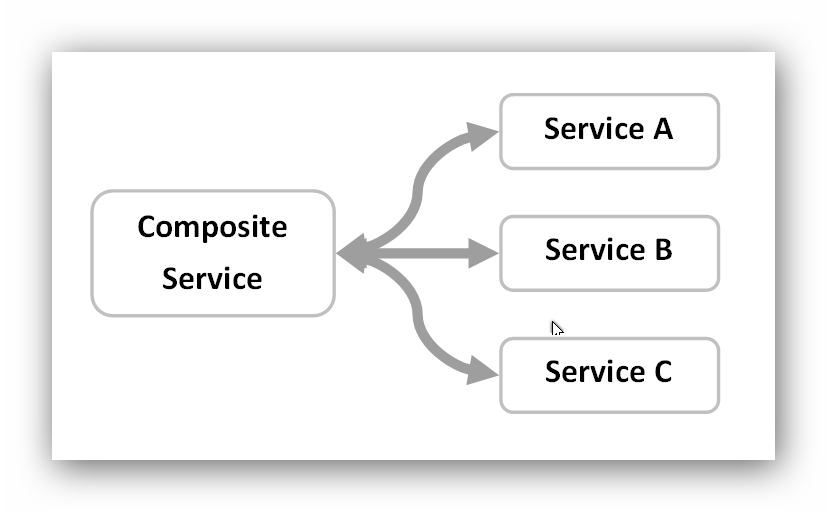
\includegraphics[width=\linewidth]{content/images/ServiceOrchestration}\
    \caption[Orchestration]{Orchestration}
    \label{fig:ServiceOrchestration}  
\end{figure}

Wie die Abbildung zeigt besteht \textbf{\underline{keine}} Verbindung zwischen:
\begin{itemize}
    \item A \& B
    \item A \& C
    \item B \& C
\end{itemize}
Nur der "`Composite Service"' nutzt die anderen Services, um den Geschäftsprozess abzubilden. Diese Art der Kommunikation nennt man Orchestration.
        
\subsection*{Choreographie}
\label{subsec:choreographie}
Anders als bei der Orchestration können Services bei der Choreographie beliebig untereinander kommunizieren. Das ist Sinnvoll, wenn verschiedene Dienste, andere Dienste über Änderungen oder andere Aktionen informieren müssen.
        
\begin{figure}[htb]
    \centering 
    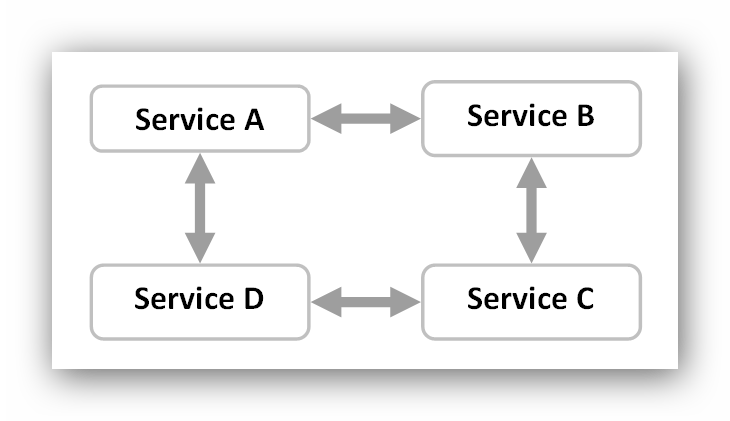
\includegraphics[width=\linewidth]{content/images/ServiceChoreography}\
    \caption[Choreographie]{Choreographie}
    \label{fig:ServiceOrchestration}  
\end{figure}